\documentclass{ximera} 
\usepackage[letterpaper, margin=.5in]{geometry}
\usetikzlibrary{math}
%----------------------------------------------------------------------------------------
%Lecture 3-1 - Intro to Polynomial Expressions
%----------------------------------------------------------------------------------------
\begin{document}
\section{Polynomial Expressions}
Before we go any deeper mathematically, we need to get some basic mechanics out of the way. You may understand concepts well, but if you can't work with polynomials then you will quickly get stuck when you try to solve problems. Nuts and bolts manipulation is omnipresent in mathematical questions.
\subsection{Monomials}
We start with the notion of a monomial.
\begin{definition}[Monomial]\index{Monomial}
	A \underline{monomial} is a single algebraic term consisting of a constant multiplied by a nonnegative integer power of one or more variables.\\
	A monomial with one variable can be written $ax^n$ where the coefficient $a$ is a real number and $n$ is a positive integer or zero.
\end{definition} 
Examples:\\
\begin{tabular*}{\textwidth}{l @{\extracolsep{\fill}} l l l l}
	$8$ & $\frac{1}{3}x$ & $-6z^{3}$ & $7a^{4}b^{9}$ & $\sqrt{7}$
\end{tabular*}\\
Notice that none of these involve addition, subtraction, or division, only multiplication.\\
\begin{example}
	A cube has side length $x$. Find monomial expressions for its volume and surface area.
		\begin{center}
		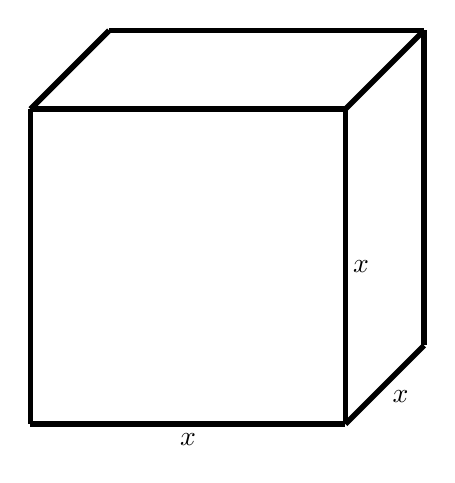
\begin{tikzpicture}[line width=2pt]
			\draw (-2,2)--(2,2);
			\draw (-2,2)--(-2,-2);
			\draw (2,2)--(2,-2);
			\draw (-2,-2)--(2,-2);
			\draw (2,2)--(3,3);
			\draw (3,3)--(3,-1);
			\draw (-1,3)--(3,3);
			\draw (-2,2)--(-1,3);
			\draw (2,-2)--(3,-1);
			\node at (2.2,0){$x$};
			\node at (0,-2.2){$x$};
			\node at (2.7,-1.65){$x$};
		\end{tikzpicture}
	\end{center}
	Volume: Volume is $\text{length}\times\text{width}\times{height}=x\cdot x \cdot x=x^3$\\
	Surface Area: Each face has area $\text{length}\times\text{width}=x\cdot x=x^2$. There are six, so the total surface area is $6x^2$
\end{example}
\subsection{Polynomial Expressions}
Monomials are the building blocks of polynomial expressions, which are what we really care about.\footnote{Well, I care anyway}
\begin{definition}[Polynomial Expression]\index{Polynomial}
	A \underline{polynomial expression} is a sum of one or more monomial expressions.\\
	A polynomial with one variable can be written
	\begin{center}
		$a_n x^n+a_{n-1}x^{n-1}+\dots+a_1 x^1 + a_0$
	\end{center}  where each coefficient $a_i$ is a real number and $n$ is a positive integer or zero.
\end{definition}
Examples:\\
\begin{tabular*}{\textwidth}{l @{\extracolsep{\fill}} l l l l}
	$x^2+4x+5$ & $-4n^5+\tfrac{5}{3}n^3-10$ & $3y-2$ & $7z^3+11z^2-z\sqrt{6}+3$ & $\tfrac{2}{7}$
\end{tabular*}\\
Notice that a single constant is technically both a monomial and a polynomial, although we don't usually think of them that way.\\ \\
There are a couple special types of polynomials that are named for the number of terms they have.\\
A \emph{binomial} is a polynomial with two terms, such as:
\begin{tabular}{l l}
	$4x-8$ & $-11z^5+z^2$
\end{tabular}\\
A \emph{trinomial} is a polynomial with three terms, such as:
\begin{tabular}{l l}
	$x^2-8x+12$ & $n^8+n-9$
\end{tabular}\\
\subsection{Terminology}
As you can probably guess, polynomials can get pretty complicated. Their different parts give us different information, so we need to introduce some vocabulary. For a polynomial 
	\begin{center}
	$a_n x^n+a_{n-1}x^{n-1}+\dots+a_1 x^1 + a_0$
\end{center}
\begin{itemize}
	\item The \emph{leading term} is $a_n x^n$
	\item The \emph{leading coefficient} is $a_n$
	\item The \emph{degree} is $n$, the highest exponent in the expression
	\item The \emph{constant term} is $a_0$
\end{itemize}
\begin{example}
	\tikzmath{
	int \a,\n,\leadco,\pdeg;
	\a4=8; \a3=5; \a2=3; \a1=13; \a0=3;
	\n4=5; \n3=3; \n2=2; \n1=1;
	\pdeg=max(\n4,\n3,\n2,\n1);
	\leadco=8;}
	Describe the characteristics of the polynomial $\a4 x^{\n4}+\a3 x^{\n3}+\a2 x^{\n2}+\a1 x^{\n1}+\a0$\\ \\
	Solution:\\
	Leading Term: $\leadco x^{\pdeg}$\\
	Leading Coefficient: $\leadco$\\
	Degree: $\pdeg$ \\
	Constant term: $\a0$
\end{example}
\begin{example}
	\tikzmath{
		int \a,\n,\leadco,\pdeg;
		\a4=7; \a3=2; \a2=13; \a1=7; \a0=23;
		\n4=6; \n3=2; \n2=8; \n1=4;
		\pdeg=max(\n4,\n3,\n2,\n1);
		\leadco=13;}
	Describe the characteristics of the polynomial $\a4 x^{\n4}+\a3 x^{\n3}+\a2 x^{\n2}+\a1 x^{\n1}+\a0$\\ \\
	Solution:\\
	Leading Term: $\leadco x^{\pdeg}$\\
	Leading Coefficient: $\leadco$\\
	Degree: $\pdeg$ \\
	Constant term: $\a0$
\end{example}
\end{document}